% !TEX root = ../thesis.tex

\vspace{-20pt}

\section{Comparative Performance Benchmarks}
\label{sec:vg:performance}

\vspace{-10pt}

To evaluate the performance of Reactive Vega against D3~\cite{bostock:d3} and
the origin, non-reactive Vega system (v1.5.0), we use the same setup described
in the previous section.

\vspace{-10pt}

\subsection{Streaming Visualizations}

\vspace{-7pt}

Figure~\ref{fig:vg:static_benchmark} shows the average performance of
uninteractive streaming scatter plots, parallel coordinates plots, and trellis
plots. We first measured the average time to initially parse and render the
visualizations. To gauge streaming performance, we next measured the average
time taken to update and re-render upon adding, modifying, or removing 1\% of
tuples. We ran 10 trials per dataset, sized 100--100,000 tuples.

\begin{figure}[t!]
  \centering
  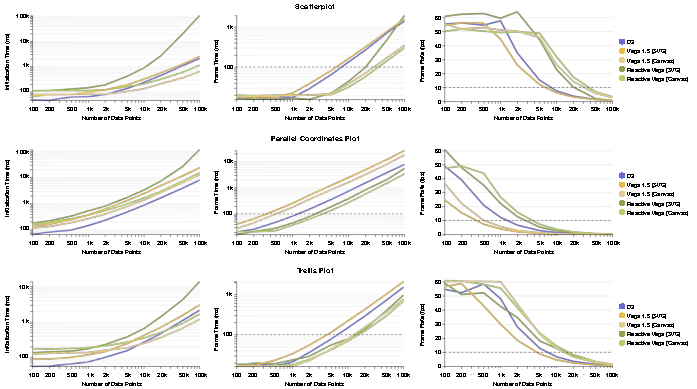
\includegraphics[width=\columnwidth]{streaming-lines.pdf}
  \caption{Average performance of rendering (non-interactive) streaming visualizations:
(top-bottom) scatterplot, parallel coordinates, and trellis plot; (left-right)
initialization time, average frame time, and average frame rate. Dashed lines
indicate the threshold of interactive updates~\cite{card:modelhuman}.}
  \label{fig:vg:static_benchmark}
\end{figure}

Reactive Vega has the greatest effect with the parallel coordinates plot,
displaying 2x and 4x performance increases over D3 and Vega 1.5, respectively.
This effect is due to each plotted line being built and encoded by its own
dataflow branch. Across the other two examples, and averaging between the Canvas
and SVG renderers, we find that although Reactive Vega takes 1.7x longer to
initialize the visualizations, subsequent streaming operations are 1.9x faster
than D3. Against Vega 1.5, Reactive Vega is again 1.7x slower at initializing
visualizations; streaming updates perform roughly op-par with the Canvas
renderer, but are 2x faster with the SVG renderer.

Slower initialization times for Reactive Vega are to be expected. D3 does not
have to parse and compile a JSON specification, and a streaming dataflow graph
is a more complex execution model, with higher overheads, than batch processing.
However, with streaming visualizations this cost amortizes and performance in
response to data changes becomes more important. In this case, Reactive Vega
makes up the difference in a single cycle.

\vspace{-10pt}

\subsection{Interactive Visualizations}

\vspace{-7pt}

We evaluated the performance of interactive visualizations (measured in terms of
interactive frame rate) using three common examples: brushing \& linking a
scatterplot matrix, a time-series overview+detail visualization, and panning \&
zooming a scatterplot. We chose these examples as they all leverage interactive
behaviors supported by D3, with canonical implementations available for
each\footnote{Brushing \& Linking:
http://bl.ocks.org/mbostock/4063663}\textsuperscript{,}\footnote{Overview +
Detail: http://bl.ocks.org/mbostock/1667367}\textsuperscript{,}\footnote{Pan \&
Zoom: http://bl.ocks.org/mbostock/3892919}. For Reactive Vega, we expressed
these visualizations with a single declarative specification. For D3 and Vega
1.5, we use custom event handling callbacks. The Vega 1.5 callbacks mimic the
behavior of the fragmented reactive approach used in prior
work~\cite{satyanarayan:declarative}. We tested these visualizations with
datasets sized between 100 and 10,000 tuples.

\begin{figure}[t!]
  \centering
  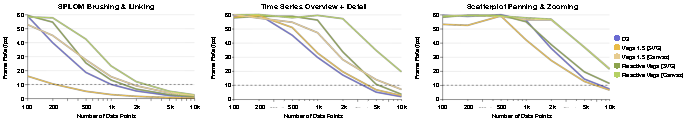
\includegraphics[width=\columnwidth]{interaction-lines.pdf}
  \caption{Average frame rates for three interactive visualizations: (left-right)
  brushing and linking on a scatterplot matrix; brushing and linking on an
  overview+detail visualization; panning and zooming on a scatterplot. Dashed
  lines indicate the threshold of interactive updates~\cite{card:modelhuman}.}
  \label{fig:vg:interactive_benchmark}
\end{figure}

Figure~\ref{fig:vg:interactive_benchmark} shows the results\,---\,on average,
and across both Canvas and SVG renderers, Reactive Vega offers superior
interactive performance to custom D3 and Vega event handling callbacks. This
effect primarily stems from Reactive Vega's unified data model, and is most
noticeable with brushing \& linking a scatterplot matrix and the time-series
overview+detail visualization. In both examples, interactions manipulate only a
subset of all data tuples. With Reactive Vega, only these tuples are processed,
and their corresponding scene graph elements re-encoded and re-rendered. In
contrast, Vega 1.5's fragmented reactive approach reconstructs and re-renders
the entire scene graph in response to changing data.